%% Included in decks: slidemage-manual, slidemage-manual-copy
%%

% SlideMage manual, chapter "Slides": versions, with SlideMage's Update version dialog
% (media/screenshot-slidemage-save-dialog.png, made by tools/manual/make_screenshots.py).
\setSlideVersion{1-0-1+}
\begin{standardframe}{Slide versions}
	\small
	A slide used in several courses changes over the years, but last year's deck
	should still compile as it was. So SlideMage keeps old versions: the file
	\SMCode{...-current.tex} is the live slide, and every \SMCode{...-v1-2-0.tex}
	beside it is a frozen copy that is never edited again. Edits are saved as you type,
	and the footer shows a ``+'' after the number (v1.2.0+) until you press \emph{Update version}
	in the Source view, which asks how big the change is:
	\par\medskip
	\begin{columns}[T,onlytextwidth]
		\begin{column}{0.42\linewidth}
			{\setlength{\fboxsep}{0pt}\fcolorbox{c_primary_gray}{white}{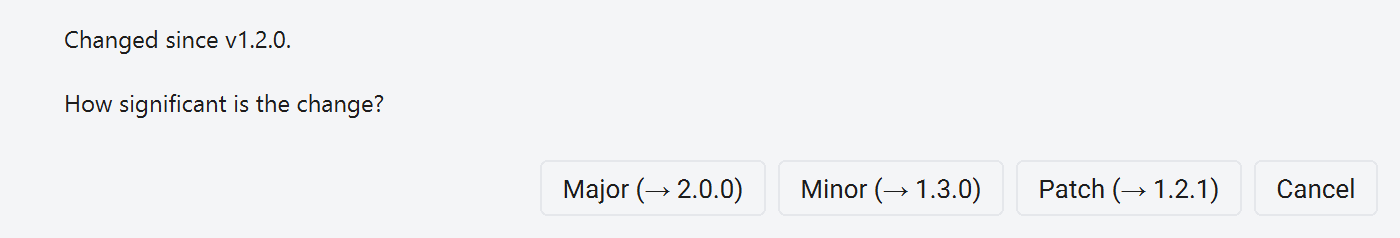
\includegraphics[width=\dimexpr\linewidth-0.8pt\relax]{media/screenshot-slidemage-save-dialog.png}}}
		\end{column}
		\begin{column}{0.54\linewidth}
			\shrinklists{1}
			\begin{itemize}
				\item \emph{Major}, \emph{Minor}, \emph{Patch}: the slide as it is now is frozen under the higher number
				\item Typo fixes need no version (the \emph{+} stays); reveal steps alone are a \emph{Patch}
				\item Several: select, right-click $\rightarrow$ \emph{Update versions\ldots}
				\item A deck keeps an old one with \SMCmd{slideversion} (\emph{Six ways to put a slide into a deck})
			\end{itemize}
		\end{column}
	\end{columns}
\end{standardframe}
